\documentclass[10pt, aspectratio=169]{beamer}

% Configuration {{{
\usepackage[utf8]{inputenc}
\usepackage[T2A]{fontenc} % T1 for English
\usepackage[english, russian]{babel}

\usepackage{mathtools}
\usepackage{graphicx}
\usepackage{tikz}
\usepackage[multidot]{grffile}
\usepackage[labelsep=period]{caption}
\usepackage{multirow}

\setbeamertemplate{caption}[numbered]
\setbeamertemplate{navigation symbols}{}
\usefonttheme[onlymath]{serif}
\usepackage{DejaVuSansCondensed} % helvet for English
\usetheme{Madrid}

\linespread{1.2}
% }}}

% Definitions {{{
\def\Dstarp{{D^{*+}}{}}
\def\Dz{{D^{0}}{}}
\def\Lc{{\Lambda_c^+}}
\def\Lcstar{{\Lambda_c^{*+}}{}}
\def\Lca{{\Lambda_c(2765)^+}}
\def\Lcb{{\Lambda_c(2940)^+}}
\def\LcII{{\Lambda_c(2625)^+}}
\def\LcIII{{\Lambda_c(2880)^+}}
\def\LcIIIother{{\Lambda_c(2765)^+}}
\def\ScI{{\Sigma_c(2455)}}
\def\ScIpp{{\Sigma_c(2455)^{++}}{}}
\def\ScIp{{\Sigma_c(2455)^{+}}{}}
\def\ScIz{{\Sigma_c(2455)^{0}}{}}
\def\ScII{{\Sigma_c(2520)}}
\def\ScIIpp{{\Sigma_c(2520)^{++}}{}}
\def\ScIIp{{\Sigma_c(2520)^{+}}{}}
\def\ScIIz{{\Sigma_c(2520)^{0}}{}}
\def\ScIII{{\Sigma_c(2800)}}
\def\ScIIIpp{{\Sigma_c(2800)^{++}}{}}
\def\ScIIIp{{\Sigma_c(2800)^{+}}{}}
\def\ScIIIz{{\Sigma_c(2800)^{0}}{}}
\def\Sc{{\Sigma_c}}
\def\Scpp{{\Sigma_c^{++}}{}}
\def\Scp{{\Sigma_c^{+}}{}}
\def\Scz{{\Sigma_c^{0}}{}}
\def\Scstar{{\Sigma_c^*}}
\def\Scstarpp{{\Sigma_c^{*++}}{}}
\def\Scstarp{{\Sigma_c^{*+}}{}}
\def\Scstarz{{\Sigma_c^{*0}}{}}
\def\Scoptstar{{\Sigma_c^{(*)}}{}}
\def\Scoptstarpp{{\Sigma_c^{(*)++}}{}}
\def\Scoptstarp{{\Sigma_c^{(*)+}}{}}
\def\Scoptstarz{{\Sigma_c^{(*)0}}{}}
\def\pip{{\pi^+}}
\def\pim{{\pi^-}}
\def\piz{{\pi^0}}
\def\rhop{\rho^+}
\def\rhom{\rho^-}
\def\Km{{K^-}}
\def\p{{p}}
\def\Dz{{D^0}}
\def\Dp{{D^+}}
\def\gevcc{{GeV$/c^2$}}
%}}}

% Title and other {{{
\title[Observation of $\ScIII$ and measurements of $\LcII$]{
  Observation of the $\ScIII$ isotriplet
  and the latest measurements of $\LcII$
  by the Belle Collaboration
  -- contents analysis
}
\author[Kerim Guseynov]{
  Kerim Guseynov \\[2ex]
  Based on
  \parbox[t]{20ex}{
    \texttt{arXiv:hep-ex/0412069}
    \texttt{arXiv:2212.04062}
  }
}
\institute[MSU]{
  Faculty of Physics \\ Moscow State University
}
\date{Dec 20, 2022}
%}}}

\begin{document}

\frame[plain]{\titlepage}

\begin{frame}[label=introduction]%{{{
  \frametitle{Introduction}
  \large
  \begin{itemize}
    \item Charm baryon resonances provide crucial tests
      for phenomenological theories.
    \item Their masses, widths are always beneficial.
    \item Decay channels are especially valuable.
    \item $\LcII$ has long been under investigation.
    \item $\LcII$ has a very small width.
      Predictions range from $0.01$ to $0.5$ MeV.
    \item Its decay channels have never been measured, either.
  \end{itemize}
\end{frame}%}}}

\begin{frame}[label=belle-detector]%{{{
  \frametitle{Belle detector}
  \centering
  \small
  Located at KEKB at KEK
  (High Energy Accelerator Research Organization, Japan)
  \vskip .5ex
  \parbox{.8\linewidth}{
    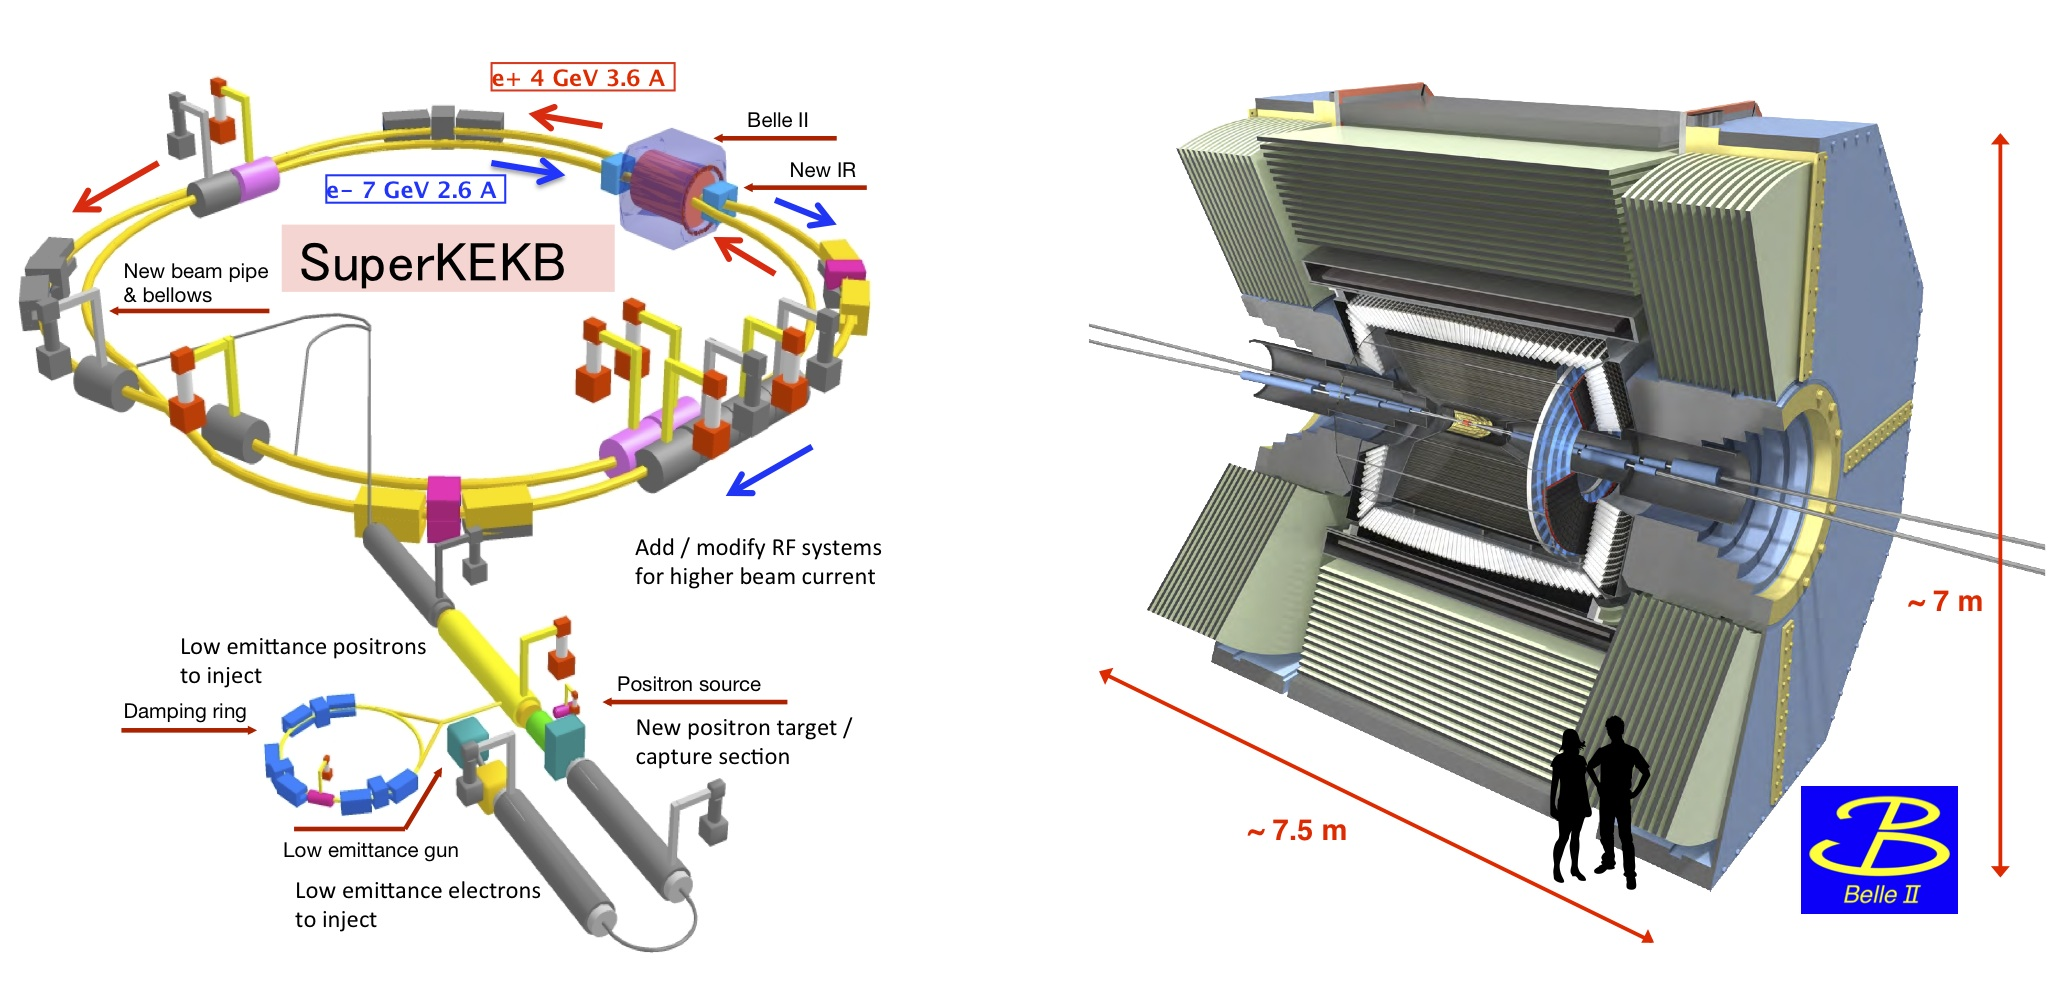
\includegraphics[width=\linewidth]{figures/004/belle-ring-detector}
  } \parbox{.19\linewidth}{
    \centering
    Vertex detector \\[1ex]
    Drift chamber \\[1ex]
    Cherenkov detector \\[1ex]
    Time-of-flight counters \\[1ex]
    Scintillator \\[1ex]
  }
  \vskip 1ex
  $ee$ annihilation at $\Upsilon(4S)$ \\[2ex]
\end{frame}%}}}

\begin{frame}[label=data-sc2800]%{{{
  \frametitle{Data selection for $\ScIII$ observation}
  $\Scstar$ resonances are observed in the $\Lc\pi^{-,+,0}$ spectra.
  \begin{itemize}
    \item $\Lc$ are reconstructed in $\Lc\to\p\Km\pip$
    \item Particle identification is based on the drift chamber, 
      time-of-flight sensors and Cherenkov detectors.
    \item PID efficiency is 83\% for protons, 84\% for kaons,
      90\% for pions.
    \item PID cuts reduce background to 3\%, 13\%, 53\%, respectively.
    \item $\Lc$ mass is limited to within $1.6\sigma$
      of the known value.
    \item $\piz$ are reconstructed as two electromagnetic showers
      with an inv. mass within $1.6\sigma$ of $m_\piz$.
    \item $\Lc\pi$ must carry 70\% or more of the full
      $ee$ collision energy.
    \item Kinematic cut on the direction of the $\pi$ relative
      to $\Lc\pi$ boost reduces soft pion background.
  \end{itemize}
\end{frame}%}}}

\begin{frame}[label=spectra-sc2800]%{{{
  \frametitle{$\Delta M(\Lc\pi) = M(\Lc\pi) - M(\Lc)$ spectra: an issue}
  \centering
  \parbox{.8\linewidth}{
    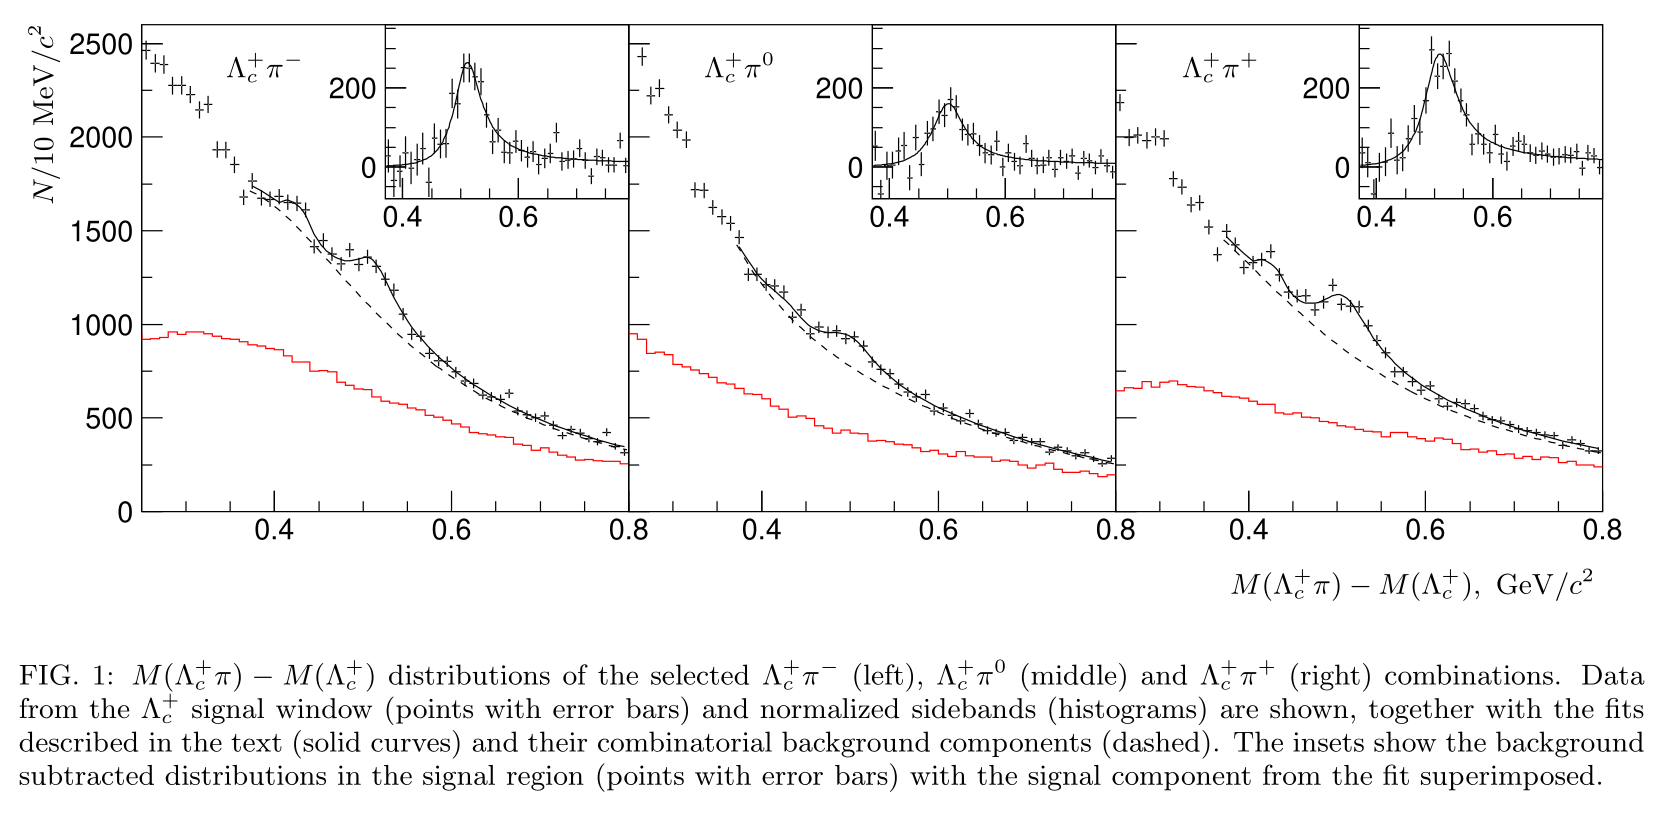
\includegraphics[width=\linewidth]{figures/005/fig1-001}
  } \parbox{.19\linewidth}{
  }
  \\[2ex] \hfill
  No features in sidebands
  \hfill
  $\LcIII$ contribution: from MC
  \hfill \null
\end{frame}%}}}

\begin{frame}[label=lcpi-from-lc2880]%{{{
  \frametitle{$\LcIII\to\Sc\pi$ component in the $\Lc\pi$ spectra}
  \centering
  \parbox{.49\linewidth}{
    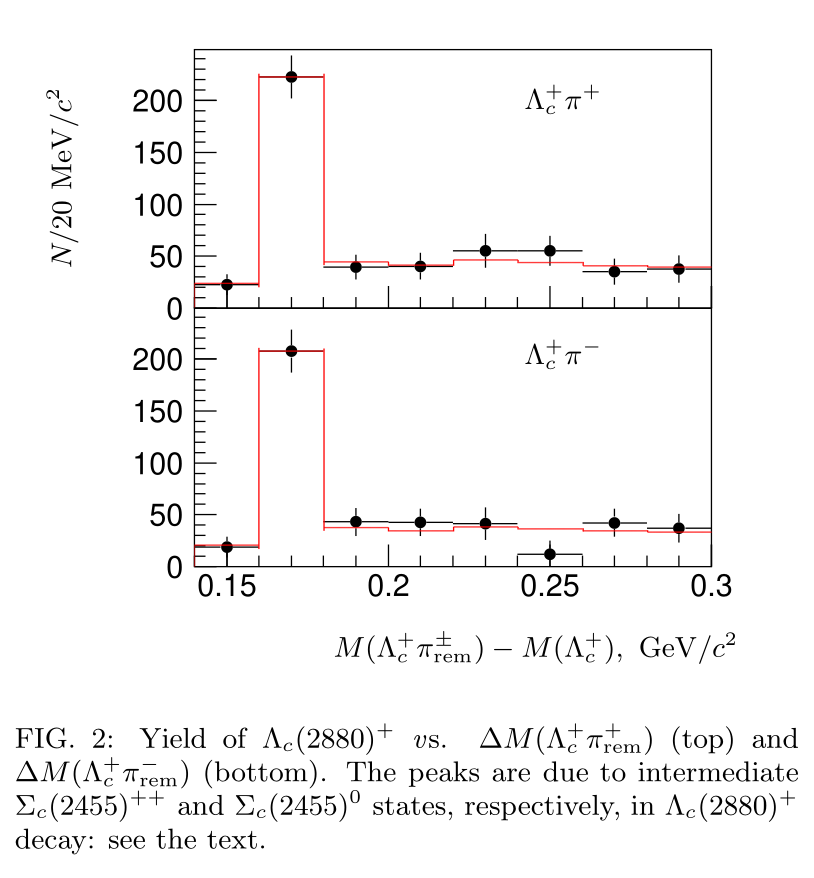
\includegraphics[height=.85\textheight]{figures/005/fig1-002}
  } \parbox{.49\linewidth}{
    $\LcIII$ contribution to $\Lc\pi$:
    \\[.5ex]
    Shape is taken from the MC.
    \\ \vfill
    Yield is also fixed in the $\Lc\pi$ fits.
    \\[.5ex]
    It is taken from $\Lc\pip\pim$ fits in bins of $\Lc\pi$.
    \\ \vfill
    30\% of events proceed via $\ScI$.
    \\ \vfill
    For $\Lc\piz$, yield is based on isospin arithmetic.
  }
\end{frame}%}}}

\begin{frame}[label=fit-sc2800]%{{{
  \frametitle{$\Delta M(\Lc\pi) = M(\Lc\pi) - M(\Lc)$ spectra and fits}
  \centering
  \parbox{.8\linewidth}{
    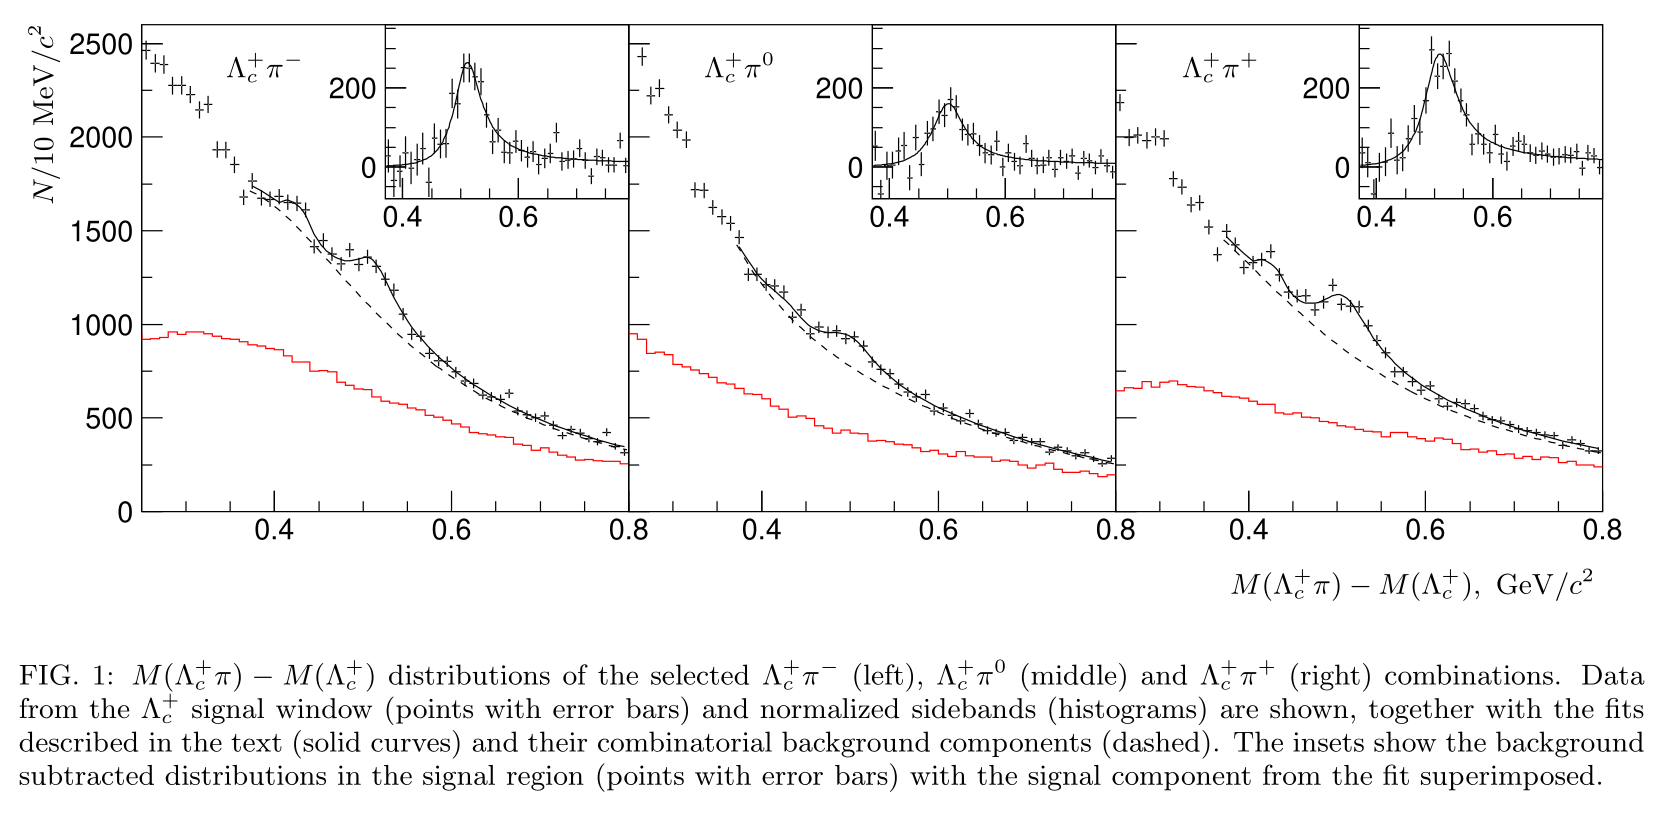
\includegraphics[width=\linewidth]{figures/005/fig1-001}
  } \parbox{.19\linewidth}{
  }
  \\[1ex] \hfill
  D-wave Breit-Wigner conv. with resolution
  \hfill
  $\LcIII$ contribution
  \hfill \null
  \\[1ex] \hfill
  3rd order inverse polynomial comb. bkg.
  \hfill \null
\end{frame}%}}}

\begin{frame}[label=systematics-sc2800]%{{{
  \frametitle{Systematic uncertainties of $\ScIII$}
  \large

  \begin{itemize}
    \item S-wave or P-wave Breit-Wigner for $\ScIII$.
    \item Extend fitting interval to the left.
    \item Comb. background model:
      \\-  Normal polynomials
      \\-  Higher and lower order inverse polynomials
      \\-  Modulated exponents
      \\-  These plus normalized $\Lc$ sidebands.
    \item Vary normalization of $\LcIII$ component within $2\sigma$.
    \item Vary momentum scale cut.
    \item Vary kinematic cut on $\pi$ angle.
  \end{itemize}

  Dominant contributions: fitting range and bkg. model.
\end{frame}%}}}

\begin{frame}[label=checks-sc2800]%{{{
  \frametitle{Checks for $\ScIII$}
  \large
  \begin{itemize}
    \item Similar structures observed in other $\Lc$ modes:
      \\- $\Lc\to p K_S^0$
      \\- $\Lc\to\Lambda^0\pip$
    \item Not reflections of higher resonances in $\Lc\pi\pi$:
      \\ these spectra exhibit no features.
  \end{itemize}
\end{frame}%}}}

\begin{frame}[label=efficiency-sc2800]%{{{
  \frametitle{Efficiencies of $\ScIII$ measurement}
  \centering
  \parbox{.48\linewidth}{
    \begin{itemize}
      \item Kinematic cut on $\pi$ direction:
        \\ $P$-parity is conserved in strong decays.
        \\ $\Lc\pi$ fits performed with kin. cuts
        complementary to the excluded region.
        \\ Corrected for detection efficiency.
      \item Momentum scale cut:
        \\ $\ScIII$ yields in bins of $x_p$.
        \\ $x_p$ spectra are extrapolated.
    \end{itemize}
  } \parbox{.48\linewidth}{
    \centering
    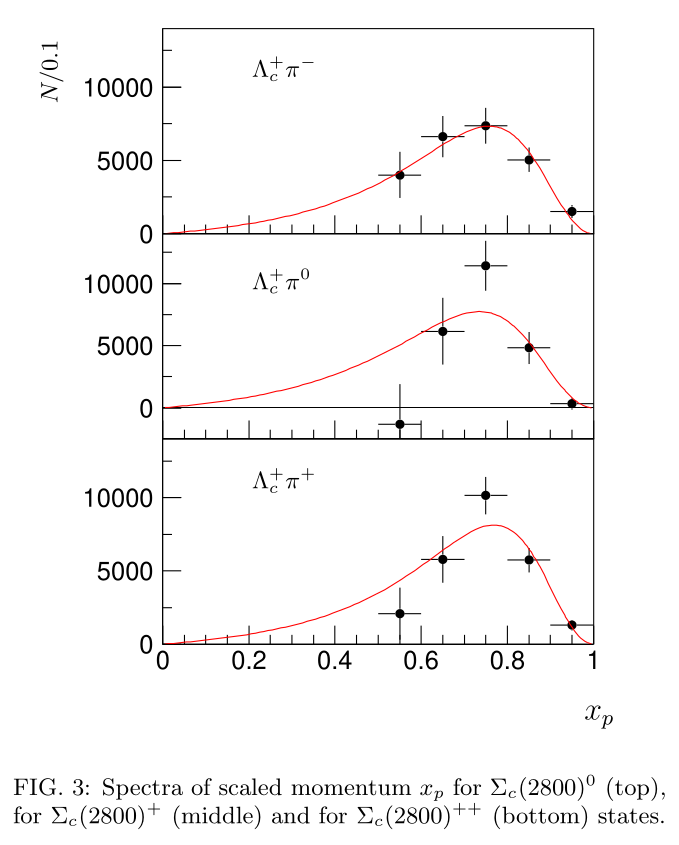
\includegraphics[height=.85\textheight]{figures/005/fig1-003}
  }
\end{frame}%}}}

\begin{frame}[label=sc2800-results]%{{{
  \frametitle{$\ScIII$ measurement results}
  \centering
  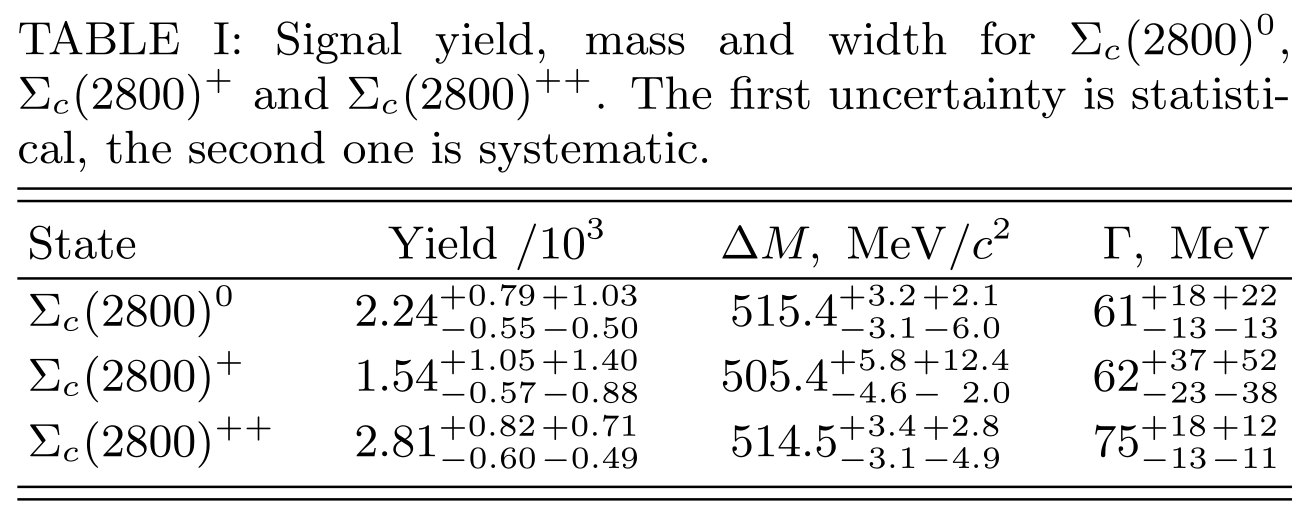
\includegraphics[width=.7\linewidth]{figures/005/tab1-001}
  \vfill
  \begin{tabular}{c l l}
    $\sigma(ee\to\ScIII X) \times \mathcal{B}\left(
      \ScIII\to\Lc\pip
    \right)=$
    & $(2.04^{+0.72}_{-0.50}{}^{+0.97}_{-0.52} \pm 0.53)$ pb & for $\ScIIIz$ \\
    & $(2.6^{+1.8}_{-1.0}{}^{+2.4}_{-1.5} \pm 0.7)$ pb & for $\ScIIIp$ \\
    & $(2.36^{+0.69}_{-0.50}{}^{+0.64}_{-0.47} \pm 0.61)$ pb & for $\ScIIIpp$ \\
  \end{tabular}
\end{frame}%}}}

\begin{frame}[label=data-lc2625]%{{{
  \frametitle{Data selection for $\LcII$ measurement}
  \begin{itemize}
    \item $\LcII$ is reconstructed in $\LcII\to\Lc\pip\pim$.
    \item $\Lc$ is reconstructed in $\p\Km\pip$.
    \item $p$, $K$, and $\pi$ are selected based on
      likelihood fits.
    \item Each of them must be 60\% to 40\% or better
      compared with alternative hypotheses.
    \item PID cuts efficiency:
      \\ 87\% for protons, 84\% for kaons, 96\% for pions.
    \item $\Lc$ mass must be within $1.6\sigma$ of the known value.
    \item $\LcII$ must carry 70\% or more of the full
      $ee$ collision enegry.
    \item Additional exp. and MC data for $\Dstarp\to\Dz\pip$,
      $\Dz\to\Km\pip$ for mass resolution.
  \end{itemize}
\end{frame}%}}}

\begin{frame}[label=resolution-lc2625]%{{{
  \frametitle{Mass resolution of $\Dstarp$ decays}
  \large
  \begin{itemize}
    \item These decays are very similar kinematically.
    \item $M(\Dz\pi) - M(\Dz)$ fit with a Breit-Wigner conv.
      with a double Gaussian function.
    \item Breit-Wigner width is fixed to the world average.
    \item Without track smearing,
      $\sigma_\text{reso}^\text{exp} /
      \sigma_\text{reso}^\text{MC} = 114\%$
    \item With track smearing,
      $\sigma_\text{reso}^\text{exp} /
      \sigma_\text{reso}^\text{MC} = 86\%$
  \end{itemize}
\end{frame}%}}}

\begin{frame}[label=lcpipi-fit]%{{{
  \frametitle{$\Lc\pip\pim$ fit with $\LcII$}
  \centering
  \parbox{.45\linewidth}{
    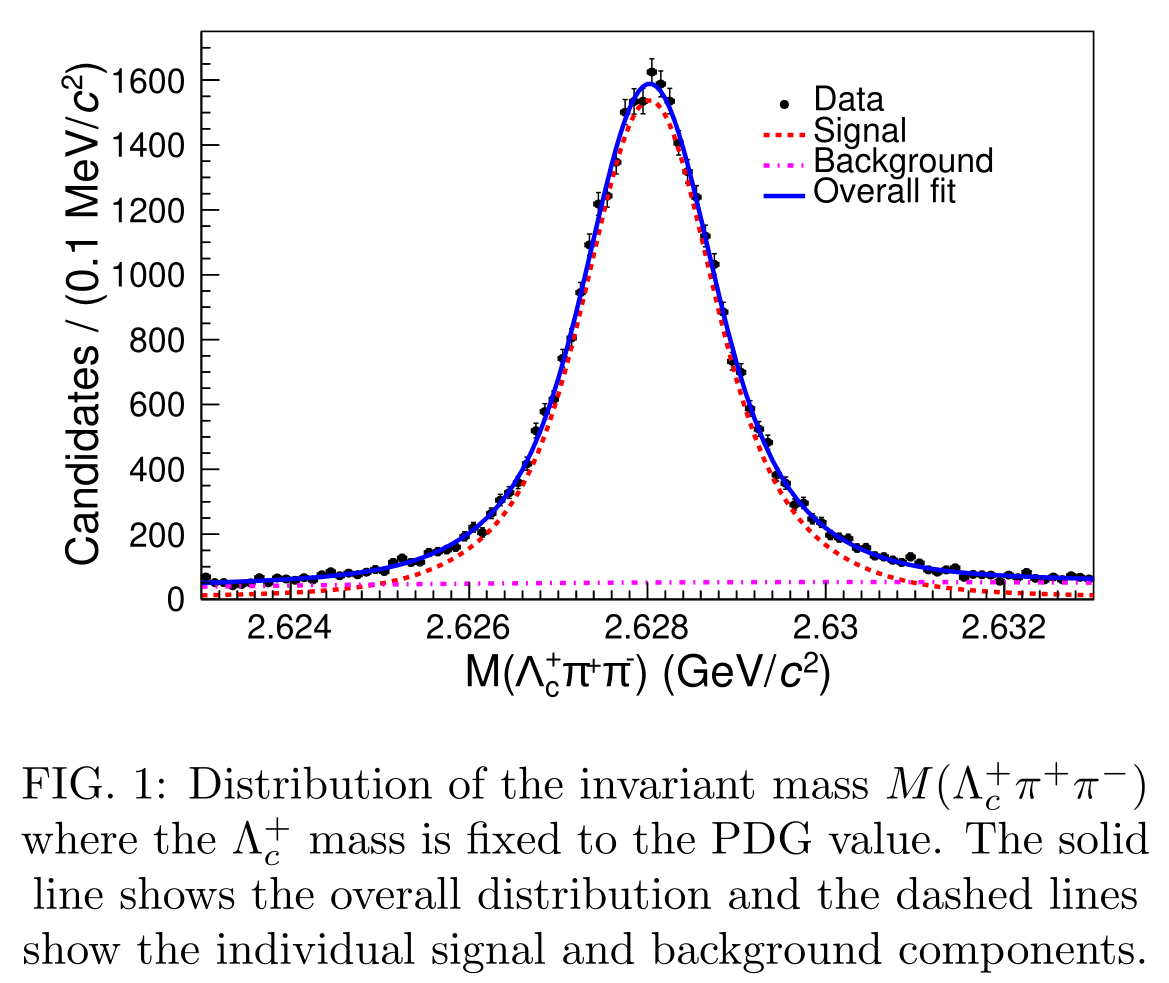
\includegraphics[width=.4\textwidth]{figures/005/fig2-001}
  } \parbox{.51\linewidth}{
    Signal is a Breit-Wigner
    \\conv. with a double Gaussian.
    \\ Bkg. is a 2nd order polynomial.
    \\[2ex]
    Resolution: \\[1ex]
    Without smearing, scaled by 114\%:
    \\ $0.490 \pm 0.025$ MeV width
    \\[1ex]
    With smearing, scaled by 86\%:
    \\ $0.293 \pm 0.026$ MeV width
    \\[1ex]
    With smearing, not scaled:
    zero natural width
    \\ \vfill
    Only an upper limit: $\Gamma(\LcII) < 0.52$ MeV
  }
\end{frame}%}}}

\begin{frame}[label=dalitz-fit-overview]%{{{
  \frametitle{Overview of Dalitz plot fit}
  \large
  \begin{itemize}
    \item Amplitude is the sum of 5 $\LcII$ decay channels:
      \\ $\ScIz$, $\ScIIz$, $\ScIpp$, $\ScIIpp$, $\Lc\pip\pim$.
    \item Bkg. described by a constant amplitude.
      \\ Different from 3-body $\Lc\pip\pim$ since the bkg.
      is flat across the Dalitz plot.
    \item Masses and widths of $\Scoptstar$ are constrained
      to the their world averages.
  \end{itemize}
\end{frame}%}}}

\begin{frame}[label=dalitz-pic]%{{{
  \frametitle{Dalitz plot in the signal region}
  \centering
  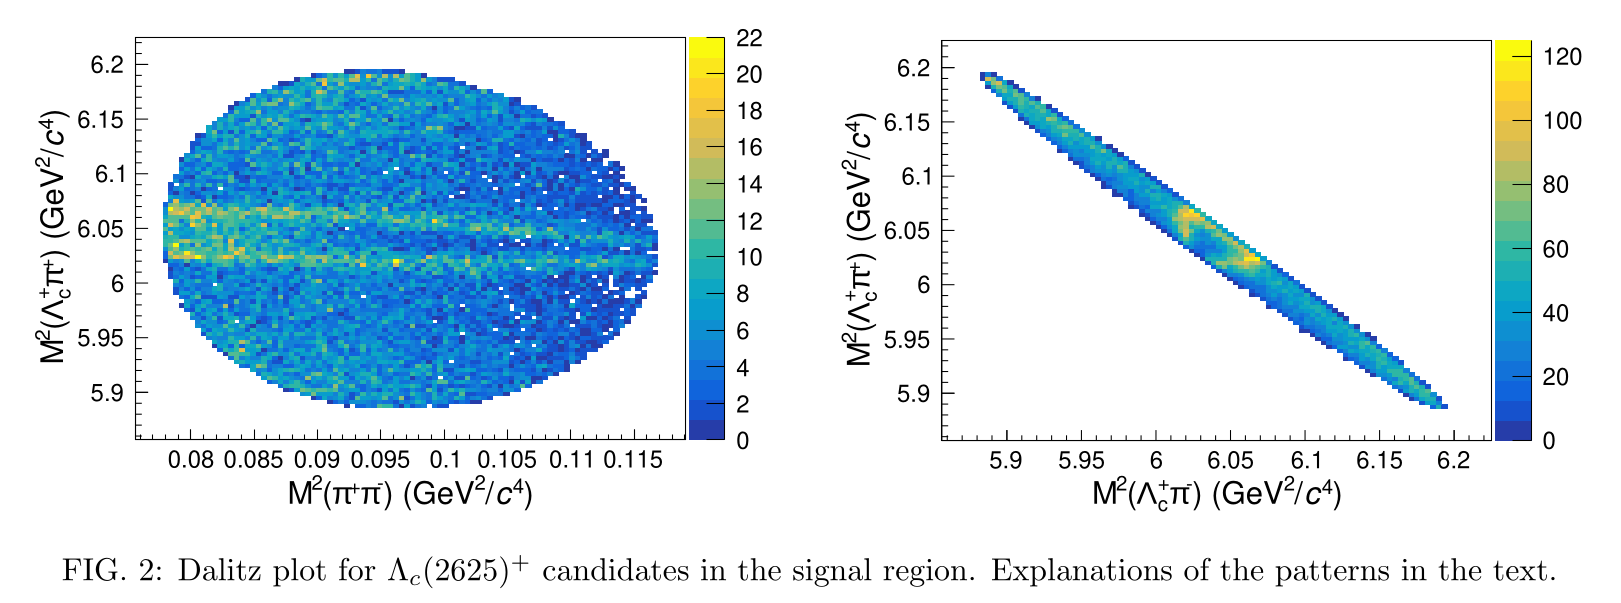
\includegraphics[width=.8\linewidth]{figures/005/fig2-002}
  \\[2ex]
  Clear $\ScIpp$ and a reflection of $\Scz$ in $\Lc\pip$.
  \vskip 1ex
  Tiny excess due to $\ScII$ at the top.
\end{frame}%}}}

\begin{frame}[label=dalitz-prj]%{{{
  \frametitle{Projections of Dalitz plot fit}
  \centering
  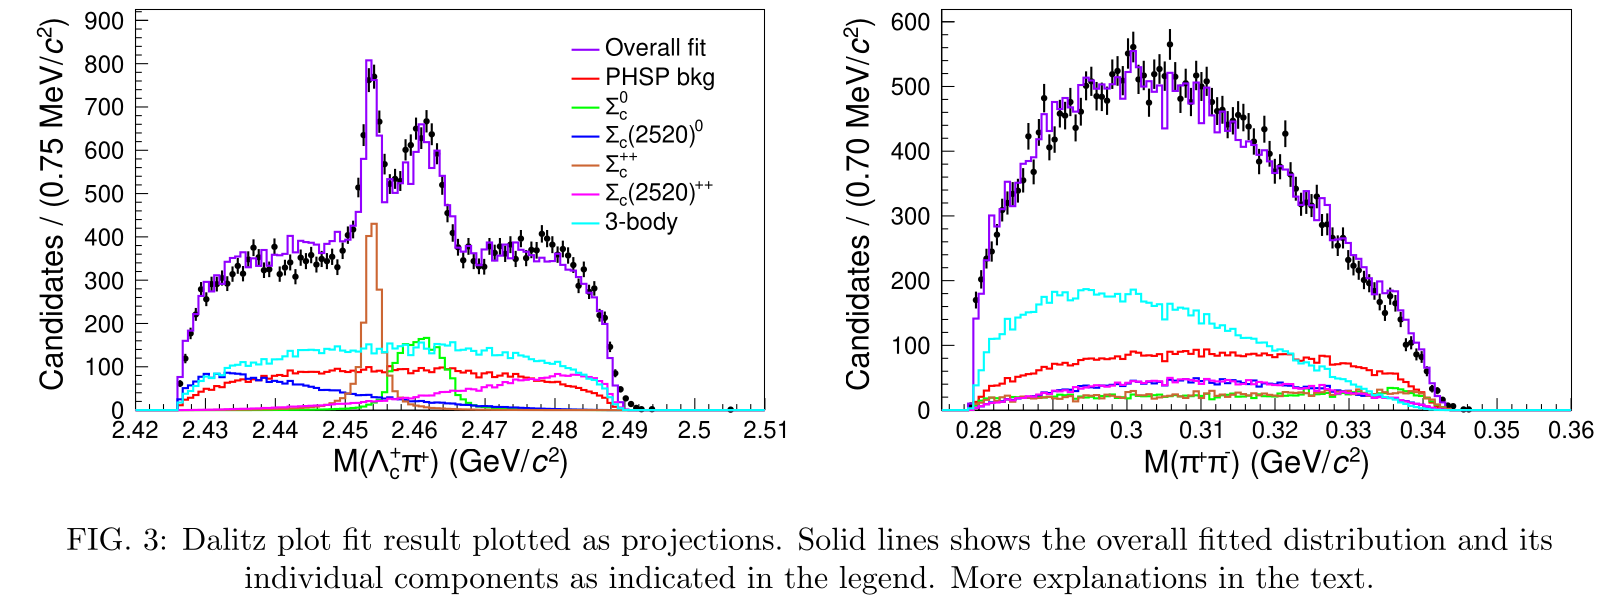
\includegraphics[width=.8\linewidth]{figures/005/fig2-003}
  \\[2ex]
  Clear $\ScIpp$ and a reflection of $\Scz$ in $\Lc\pip$, again.
  \vskip 1ex
  Small $\ScII$ on the sides in $\Lc\pip$.
  \hspace{4ex}
  $\Lc\pip\pim$ is asymm. while bkg. is simm. in $\pip\pim$.
  \vskip 1ex
  Yields of $\LcII$, $\ScIpp$, $\ScIz$ obtained.
  \hspace{4ex}
  Not all $\ScI$ come from $\LcII$.
\end{frame}%}}}

\begin{frame}[label=dalitz-lc2625-sidebands]%{{{
  \frametitle{Dalitz plot fits of $\LcII$ sidebands}
  \parbox{.48\linewidth}{
    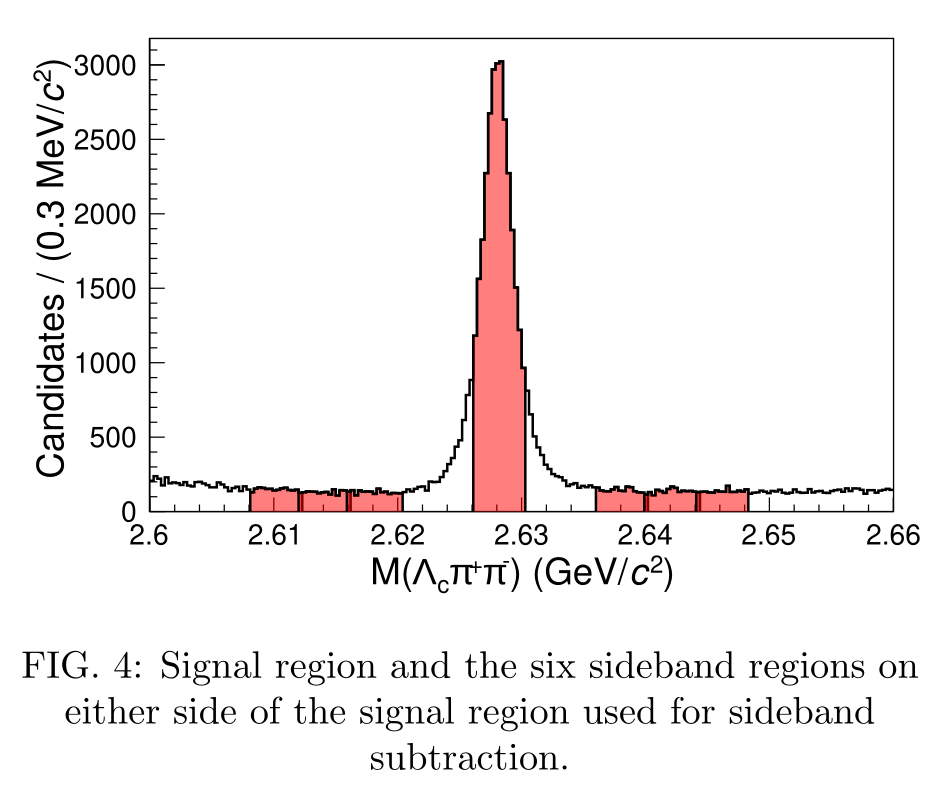
\includegraphics[width=\linewidth]{figures/005/fig2-004}
  } \parbox{.48\linewidth}{
    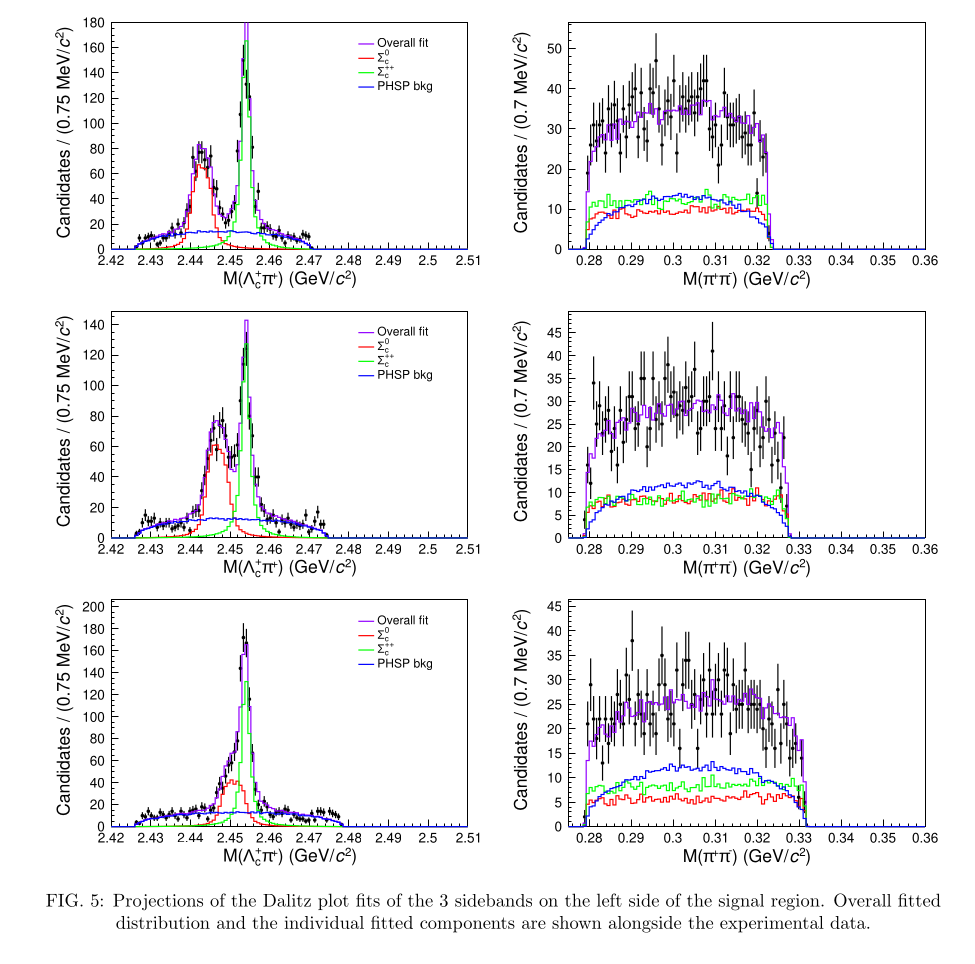
\includegraphics[width=\linewidth]{figures/005/fig2-005}
    %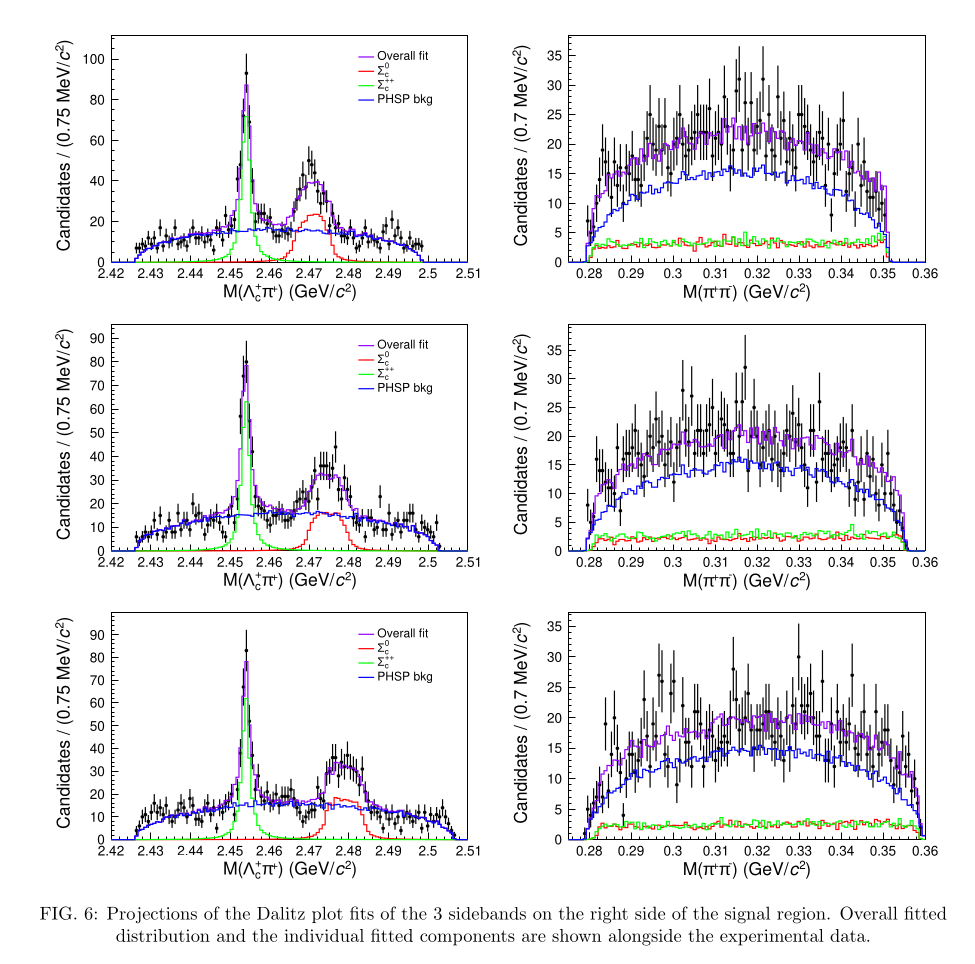
\includegraphics[width=\linewidth]{figures/005/fig2-006}
  }
\end{frame}%}}}

\begin{frame}[label=lc2625-sidebands-extrapol]%{{{
  \frametitle{$\ScI$ yields extrapolation from $\LcII$ sidebands}
  \centering
  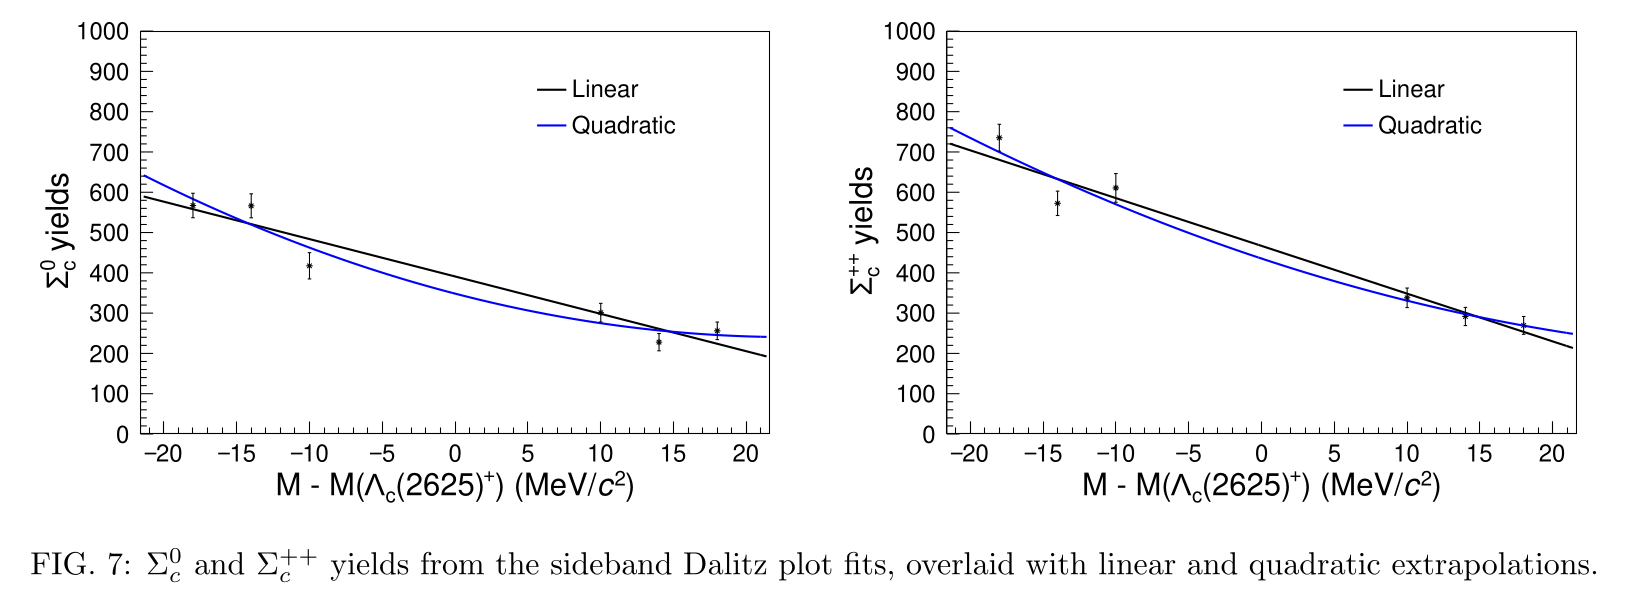
\includegraphics[width=.8\linewidth]{figures/005/fig2-007}
  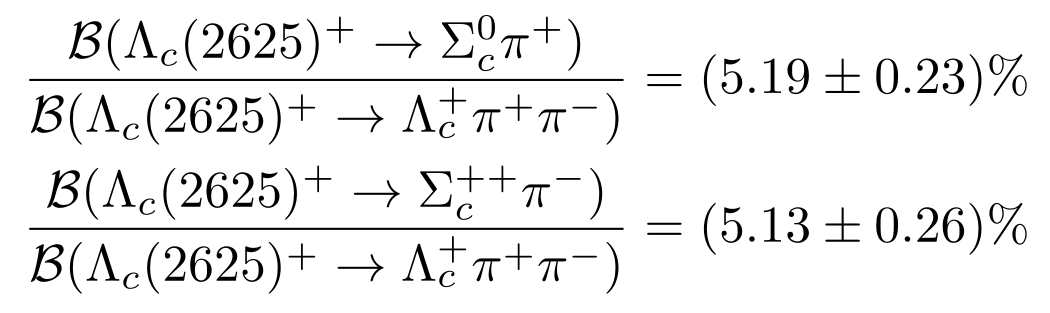
\includegraphics[width=.4\linewidth]{figures/005/lc2625-br-statonly}
\end{frame}%}}}

\begin{frame}[label=systematics-lc2625]%{{{
  \frametitle{Systematic uncertainties of the $\LcII$ measurement}
  $\LcII$ mass precision is limited by Belle capabilities.
  \begin{itemize}
    \item Based on $\Dstarp$ decays, soft pions are calibrated
      so that $m_\Dstarp$ matches the world average.
    \item Applying this calibration to $\LcII$ shifts its mass.
    \item Belle also corrects low momenta, which slightly affects
      the mass measurement.
  \end{itemize}

  $\LcII$ branching ratios uncertainties come from
  \begin{itemize}
    \item $\LcII$ yield itself, $\ScIpp$ and $\ScIz$ yields
      and bkg. corrections.
    \item $\LcII$ yield is most affected by the mass resolution.
    \item Masses and widths of $\ScI$ are varied within
      world average errors.
    \item Linear or quadratic extrapolation for $\ScI$
      yield corrections.
    \item The finite MC sample size is also a source.
  \end{itemize}
  %\hfill 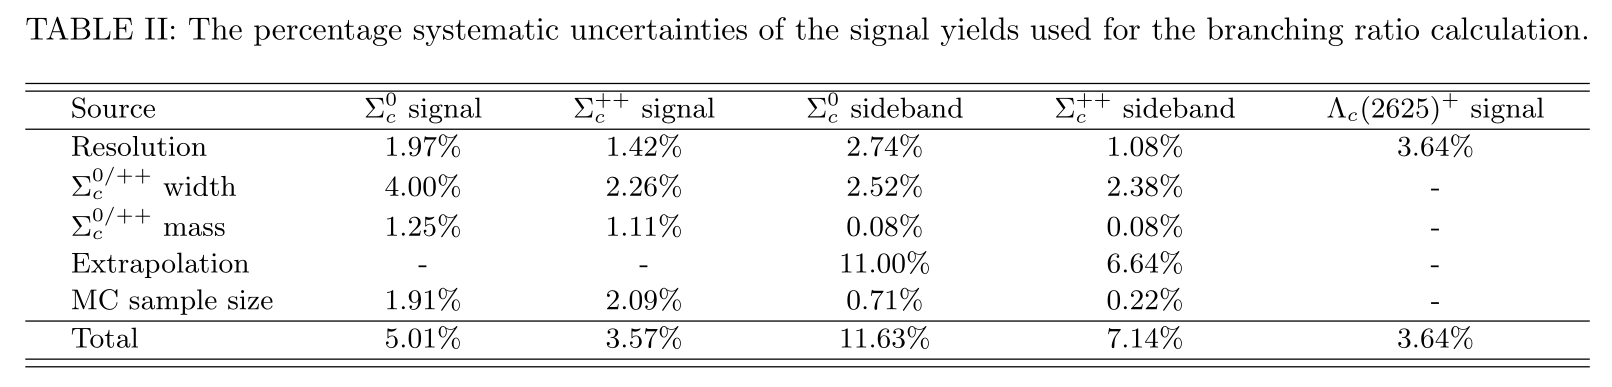
\includegraphics[width=.8\linewidth]{figures/005/tab2-002} \hfill\null
\end{frame}%}}}

\begin{frame}[label=lc2625-results]%{{{
  \frametitle{$\LcII$ measurement results}
  \begin{itemize}
    \item $\LcII$ mass measurement is the most precise yet
      and is consistent with previous ones
      $$ m_\LcII = 2627.978 \pm 0.006 \pm 0.049 \text{ MeV} $$
    \item $\LcII$ width upper limit is the smallest yet
      $$ \Gamma_\LcII < 0.52 \text{ at 90\% C.L.} $$
      Some predictions are ruled out,
      but higher precision is required.
    \item $\LcII$ branching ratios extracted from
      a full Dalitz plot fit are their first measurements
      $$ \frac{\mathcal{B}\left(\LcII\to\ScIz\pip\right)}
      {\mathcal{B}\left(\LcII\to\Lc\pip\pim\right)}
      = (5.19 \pm 0.23 \pm 0.40)\%$$
      $$ \frac{\mathcal{B}\left(\LcII\to\ScIpp\pim\right)}
      {\mathcal{B}\left(\LcII\to\Lc\pip\pim\right)}
      = (5.13 \pm 0.26 \pm 0.32)\%$$
  \end{itemize}
\end{frame}%}}}

\end{document}
